
\section{\sys{} Agentic Architecture}
\label{sec:design}

\begin{figure}[t]
   \centering
   \noindent\hspace*{-6pt}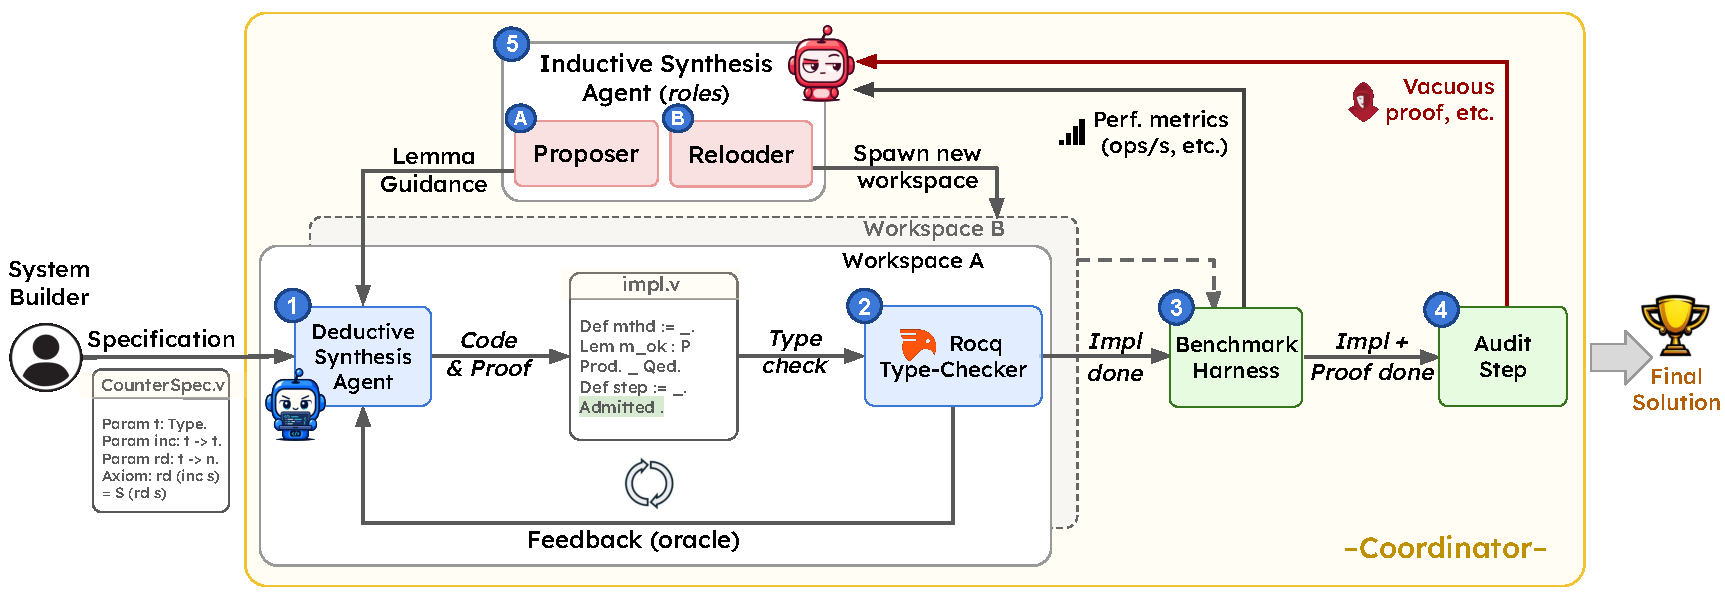
\includegraphics[width=\dimexpr\linewidth+12pt\relax]{figures/OVERVIEW_final.pdf}\hspace*{-6pt}
   \caption{\sys{}' agentic architecture; code and proof advance jointly throughout. A coordinator runs parallel \fignum{1} Deductive Synthesis Agents (DSAs); each step is graded by \fignum{2} \coq{}'s type-checker, completed implementations are \fignum{3} benchmarked, and closed proofs are \fignum{4} audited for non-vacuity. On failure, the \fignum{5} Inductive Synthesis Agent (ISA) intervenes: \fignum{A} \emph{proposer} adds helper lemmas on tactical stalls; \fignum{B} \emph{reloader} respawns a DSA with a fresh design on strategic dead-ends.
% \mohsen{Can we add 5 and 6 for proposer and reloader as well?} \shubham{Addressed: \fignum{5} for ISA, \fignum{A} for proposer, \fignum{B} for reloader (matching the figure's 5 / A / B labels).}
}
   % \mohsen{Strategist Agent -> Inductive Synthesis Agent}}
   \label{fig:architecture}
\end{figure}
% \shu{can we even make the specification and the code generation block larger? Audit step is done by an agent right? should we have a role there?}
% \mert{there is a lot of unused empty space, perhaps the figure can be arranged to make the code and writings look larger?}
% \mohsen{The text needs to be larger.}

% \accheng{can we try to structure the text to be more readable? the paragraphs are too dense right now and hard to get what the main takeaways are. I would try to highlight insights, key design decisions, etc. Right now, it reads more like a description of an implementation}

\textbf{Overview. \ }
%
We now describe how we realize IDS as an agentic architecture (\cref{fig:architecture}). Given a system interface and property specifications, the framework orchestrates multiple LLM agents guided by verification and performance feedback to generate an efficient, mechanically-checked implementation. This architecture relies on a powerful synergy: deductive synthesis constructs the code and proof under a given strategy, while inductive synthesis discovers better strategies from failed attempts.
% This paper realizes IDS as an agentic certified synthesizer.
% 
% Our framework takes as input the signature of a distributed key-value-store implementation and the specification of its properties.
% It then uses multiple LLM agents, with a proof assistant providing verification feedback,
% and a benchmark harness providing performance feedback,
% to generate an efficient implementation
% paired with a mechanically-checked proof that it satisfies the specification.
% Deductive and inductive synthesis form a powerful combination:
% % deductive synthesis produces rigorous proofs,
% % and inductive synthesis discovers effective proof strategies.
% % Deductive and inductive synthesis combine naturally in IDS: 
% given a strategy, deductive synthesis constructs an implementation and a machine-checked proof; 
% given failed attempts, inductive synthesis discovers more effective strategies.

% Inspired by deductive synthesis~\cite{manna-waldinger,manna2006synthesis}, \sys{} introduces Deductive Synthesis Agents (DSAs, \fignum{1}) to incrementally synthesize implementations from specifications. Guided by a strategy, a DSA decomposes a component into sub-components. It inserts placeholders for these sub-components to construct the parent implementation, simultaneously decomposing the parent specification into corresponding sub-specifications. This step leverages both the specification's structure (\ie a specification composed of multiple methods naturally splits into separate specifications for each method) and the LLM's knowledge of decomposition patterns. Assuming the sub-components satisfy their sub-specifications, the DSA constructs the proof of correctness for the parent component. This recursive process repeats until the search tree reaches trivial sub-components and sub-specifications. The agent applies a similar approach to decompose lemmas into helper lemmas. At every step, it uses the \coq{} type-checker (\fignum{2}) to verify the correctness of both complete and partial proofs.

Inspired by deductive synthesis~\cite{manna-waldinger,manna2006synthesis}, \sys{} introduces Deductive Synthesis Agents (DSAs, \fignum{1}) to incrementally synthesize implementations from specifications. Guided by a strategy, a DSA recursively decomposes a component and its specification into sub-components using placeholders. 
% Leveraging the LLM's structural knowledge, 
The DSA constructs proofs assuming these sub-components are correct, repeating this process down to trivial elements. The \coq{} type-checker (\fignum{2}) continuously verifies both complete and partial proofs throughout this decomposition.

% Inspired by deductive synthesis~\cite{manna-waldinger,manna2006synthesis},
% \sys{} introduces Deductive Synthesis Agents (DSAs, \fignum{1})
% that incrementally synthesize the implementation from the specification.
% Given a strategy, 
% a DSA decomposes the synthesis of a component into the synthesis of sub-components.
% It sets placeholders for implementations of sub-components
% and constructs an implementation of the component using the sub-components.
% It further
% decomposes the specification of the component into sub-specifications for the sub-components.
% It draws on both the specification's structure (\ie a specification composed of multiple methods naturally splits into separate specifications for each method) and the LLM's knowledge of decomposition patterns.
% Assuming sub-components satisfy their sub-specifications,
% it constructs the proof of correctness for the component.
% It then repeats the process for sub-components.
% The process terminates when the search tree reaches trivial sub-components and sub-specifications.
% It takes a similar approach in decomposing lemmas into helper lemmas.
% It uses the type-checker of \coq{} (\fignum{2}) to check the correctness of complete as well as partial proofs at each step.
% decomposed specifications of its sub-components.
% \shu{step 3 is missing, overview is way, way too long... it is very hard to parse, can we make it shorter?}
% DSA proves effective when driven the right path.


% A DSA is effective when guided by a good search strategy\shu{is strategy defined somewhere? what is strategy? is it code?}, such as introducing the right ghost state
% (an auxiliary variable that is added to captures an invariant).
% However, with a dead-end strategy, a DSA may get stuck taking steps without closing the proof.
%
% \accheng{do you already explain what CEGIS is before? I wouldn't assume reviewers are familiar} \shubham{Could name the counterexample at the inner DSA level as the structured \coq{} error trace (\cref{app:feedback}); FB ablation in \cref{sec:eval-ablations} confirms the trace, not just a binary verdict, carries the signal.}
% In the spirit of inductive synthesis, 
% Inspired by inductive synthesis~\cite{cegis,sketch,clarke2000counterexample}, \sys{} introduces an Inductive Synthesis Agent (ISA, \fignum{5}) that learns from failed strategies and proposes more promising ones. 
% It is given feedback
% when a DSA stalls at a proof attempt and 
% when the performance is evaluated.
% The ISA plays two roles, \emph{proposer} (tactical, \fignum{A}) and \emph{reloader} (strategic, \fignum{B}). \shu{what is tactical and strategic?}
% A DSA is effective when guided by a sound search strategy, which represents a high-level design or proof approach such as introducing the right ghost state (an auxiliary variable used to capture an invariant). However, under a dead-end strategy, a DSA may get stuck taking steps without closing the proof. 
% Inspired by inductive synthesis~\cite{cegis,sketch,clarke2000counterexample}, \sys{} introduces an Inductive Synthesis Agent (ISA, \fignum{5}) that learns from failed strategies and proposes more promising ones. The ISA receives feedback when a DSA stalls at a proof attempt and when system performance is evaluated. The ISA plays two roles: a \emph{proposer} for tactical, local adjustments to the current approach (\fignum{A}), and a \emph{reloader} for strategic, global shifts to entirely new designs (\fignum{B}).

While this deductive approach succeeds when guided by a sound search strategy (e.g., a high-level design or proof approach in the prompt), a DSA can stall under a dead-end strategy. Inspired by inductive synthesis~\cite{cegis,sketch,clarke2000counterexample}, \sys{} introduces an Inductive Synthesis Agent (ISA, \fignum{5}) that learns from failed strategies to propose more promising ones. The ISA receives feedback when a DSA stalls or yields poor performance. It then intervenes in two roles: a \emph{proposer} for tactical, local adjustments (\fignum{A}), and a \emph{reloader} for strategic, global shifts to entirely new designs (\fignum{B}).

% informed of a failed strategy
% Here the role of the counterexample is played by two negative signals to the ISA: 

\textbf{Coordinator. \ } The coordinator launches and orchestrates the DSAs and the ISA, maintaining overall system state and managing a parallel pool of workers. While DSAs can report localized errors, they cannot detect strategic dead-ends on their own. The coordinator monitors progress to identify stagnating agents, recording failed strategies and invoking the ISA to propose new ones before respawning the DSA. 
 
To ensure the synthesized system is not only correct but also performant, the coordinator benchmarks each candidate eagerly, even before its proof completes. It extracts the implementation to executable code and runs the benchmark harness (\fignum{3}, \cref{sec:eval-setup}). The measurements are fed back to the ISA so that its future strategies guide the DSA toward more efficient implementations. Once a proof closes (i.e., the proof completes with no remaining \texttt{Admitted} placeholders), the coordinator audits the result to ensure it is fully verified, non-trivial, and implements the expected interface (\fignum{4}). Finally, it returns the most efficient verified solution found within the time budget. 
% Next, we consider the DSA and ISA more closely.


% \sys{} presents a coordinator that orchestrates the DSAs and the ISA.
% \textbf{Coordinator. \ }
% The coordinator launches and orchestrates the DSAs and the ISA, and maintains state. The coordinator starts with one DSA and grows a pool of DSAs in parallel over time.
% In order to avoid the sunk-cost fallacy, the DSA reports when it is stuck with a repeating error; however, it cannot tell when it faces a strategic dead-end. Therefore, the coordinator periodically polls each DSA and tracks the number of open and finished proofs. 
% If it deems that a DSA is stagnating,
% it records the failed strategy,
% and invokes the ISA
% to either revise the strategy, or propose a new one.
% It then respawns the DSA with that strategy, or spawns an additional DSA.
 

% The coordinator benchmarks each candidate eagerly, 
% even before its proof completes.
% The coordinator extracts the implementation to executable code,
% % from Gallina to OCaml
% and runs the benchmark harness (\fignum{3}, \cref{sec:eval-setup}).
% The measurements are fed back to the ISA
% so that its future strategies
% guide the DSA toward more efficient implementations.
% % 
% % Finally, the coordinator returns the most efficient verified solution
% % that was found in the time budget.
% The coordinator
% runs the audit step (\fignum{4}) when the proof closes.
% In addition to type-checking, it checks that (i) no assumptions
% % \texttt{Axiom}/\texttt{Hypothesis}/\texttt{Parameter}/\texttt{Admitted} 
% remains in the final output, (ii) the expected interface is implemented, (iii) the implementation is non-trivial, and (iv) the proper correctness statement is included.
% % 
% Finally, it returns the most efficient verified solution
% found within the time budget.
% 
% 
% coordinator, 
% Next, we consider the DSA and ISA more closely. \shu{this is very long, some of the details in the first paragraph is about implementation right? imo we should have a shorten overview that includes all points, and dive into specific agents in subsequent paragraphs}
% in turn.

% Worker holds proof state across many turns while Meta sees only summaries -- separating context windows lets Worker stay deep without Meta drowning in tokens


% \mert{
% Overall, this multi-agent archiecture needs to be well motivated. It should not feel like this archiecture is vibe-coded, abut there is an essential need and a natural nreason behind these agentic roles. Also it is not super clear if \emph{Heartbeat} is an agent or not, the difference between the \emph{Guide} and \emph{Resetter} or \emph{Meta}.
% Why cant these be a single agent that is equipped to do multiple responsibilities given different situations for example? Context management can be a key reason, but needs to be motivated.} 
% \accheng{agree, providing some high-level motivation for the overall architecture will make it more convincing}
% \shubham{Can add a ``Why multi-agent'' opener: (a) Heartbeat is deterministic Python (not an LLM), so ``DONE'' is a kernel-level verdict not another model output; (b) Worker holds proof state across many turns while Meta sees only summaries -- separating context windows lets Worker stay deep without Meta drowning in tokens; (c) Guide/Resetter are different decision horizons (tactical vs strategic) and a single agent making both calls in one prompt empirically picks the wrong move when the failure mode is mixed.}


% % ------------------------------------------------------
% \textbf{Coordinator. \ }
% % \subsection{Monitor}
% \label{sec:design-heartbeat}
% % 
% The coordinator is a program that launches the agents, maintains state, and coordinates them. It is deterministic Python rather than an LLM, so its verdicts (a DSA is stagnating; a candidate is audit-clean) are kernel-level rather than model outputs. It starts with one DSA and grows the pool over time, with each DSA exploring a different synthesis tree in its own sandboxed workspace. 
% The DSA reports when it is stuck with a repeating error; however, it cannot tell when it faces a strategic dead-end. Therefore, the coordinator polls each DSA every $5$ minutes and tracks the number of open and finished proofs (\ie \texttt{Admitted} and \texttt{Qed} terms): if neither count has changed across $10$ consecutive polls, the DSA is flagged as stagnating, and the coordinator invokes the ISA with the previous strategies, escalating with a new ISA invocation every $20$ further polls of continued stagnation. The ISA then refines the current strategy or proposes a new one. The coordinator provides the DSA with the refined strategy, respawns it with the new one, or spawns an additional DSA in a new workspace.
% 
% The coordinator empirically evaluates not only a DSA's verified solutions but also implementations whose proof is incomplete.
% This eager evaluation helps avoid verifying an implementation that is slower than previously-known candidates.
% The coordinator extracts the implementation to executable code,
% % from Gallina to OCaml
% and runs the benchmark harness (\cref{sec:eval-setup}).
% % If the implementation is slow,
% It then passes the performance feedback to the ISA, which gives the DSA a new strategy.
% %
% When a DSA closes the proof, the coordinator runs the audit step: in addition to type-checking, it checks that the expected interface is implemented, the implementation is non-trivial, and the proper correctness statement is included. If the audit step rejects the candidate (e.g., a vacuous proof), it is sent to the ISA.
% %
% % The coordinator returns the best known solution or failure when the allocated time is over.
% The coordinator returns the best solution found, or reports failure, upon exhausting the time budget.
% 
% % \item \textbf{If Meta itself stagnates.} If Meta's interventions yield no new \texttt{Qed} across $N$ consecutive heartbeats, Heartbeat fires a one-shot Meta-Meta call: a higher-level invocation that reads Meta's prior guidance and proposes a strategy Meta has not yet tried.



\textbf{DSA: Deductive Synthesis Agent. \ }
% \subsection{DSA: Deductive Synthesis Agent}
\label{sec:design-worker}
Off-the-shelf LLMs, pretrained on a large corpus of programs and proofs, are well-equipped to guide synthesis search,
as we empirically demonstrate in \cref{sec:eval-synthesis}. To harness this capability, we design the DSA as a generic LLM coding agent operating under strict constraints: implementations must be well-typed before proving, specifications cannot be altered, final outputs must contain no unproven assumptions, and system state must remain bounded.

% Pretrained on a large corpus of programs and proofs,
% off-the-shelf LLMs are well-equipped to guide the synthesis search,
% as we empirically demonstrate in \cref{sec:eval-synthesis}.
% A DSA is a generic headless LLM coding agent (Codex, Claude Code) with the following briefings.
% % 
% \emph{Methodology.} 
% % Plan the implementation before writing code.
% The implementation should be well-typed before attempting a proof.
% The refinement relation between the states of the implementation and specification should be explicitly written and type-checked.
% % non-simulation obligations (initialisation, preservation, parametricity) are discharged before the main simulation theorem.
% % 
% \emph{Auditability.} 
% The specification shouldn't be changed.
% No assumptions
% % \texttt{Axiom}, \texttt{Hypothesis}, \texttt{Parameter}, or \texttt{Admitted} 
% should be in the final output.
% % 
% \emph{Design.}
% The declared system state should not grow unboundedly with the number of operations.
% 
% \item
% \emph{Tactical playbook.} Use the curated set of tactic patterns from interactive-proof practice (\cref{app:proof-method}).

At each node of the search tree, the agent can take the following actions to advance the synthesis: (1) define partial implementations, (2) close open proof branches, or (3) decompose complex lemmas into simpler helper lemmas. After each step, the implementation and proof are passed to \coq{}'s type-checker. If there are no errors, the state is saved, building a search tree of well-typed partial implementations and proofs. If errors occur, the agent can take the following actions: (1) repair the failed step by attempting a different approach, or (2) revert to an earlier node in the search tree.

% % The DSA is \sys's deductive-synthesis agent: 
% Given a specification, a DSA incrementally refines it into an implementation.
% % and a machine-checked proof that the implementation satisfies the specification.
% % The specification declares the interface to implement and the properties the implementation must satisfy.
% % The agent 
% In order to synthesize a component, it chooses a strategy, generates placeholders for the required sub-components, and implements the component using the sub-components.
% Accordingly, it decomposes the specification into sub-specifications for sub-components, drawing on both the spec's structure (a spec composed of multiple methods naturally splits into per-method obligations) and the LLM's knowledge of decomposition patterns.
% It then assumes that the sub-components will satisfy the sub-specifications, and
% constructs a proof that the implemented component satisfies its specification.
% In the next iterations, the agent continues to synthesize
% % implementations of the 
% sub-components that satisfy the sub-specifications.
% % Finally, the search tree culminates in trivial sub-components and sub-specifications.
% The process terminates when the search tree reaches trivial sub-components and sub-specifications.
% 
% At each node of the search tree, the agent can take the following actions.
% % each step of the search
% (1) \emph{Define}: 
% Declare, refine or extend a state or message type, or function body. Partial function definitions can be written with placeholders (\ie \texttt{admit}) which are tackled in the next steps.
% % 
% (2) \emph{Prove}:
% Close an open proof obligation (\ie replace \texttt{Admitted} with \texttt{Qed}) or extend the proof with more tactics.
% % 
% (3) \emph{Decompose}:
% State and assume helper lemmas (\ie as \texttt{Admitted}) which are tackled in the next steps. Then, use the helper lemmas to advance the proof of existing lemmas.
% % 
% After each of the above steps,
% the implementation and proof
% are passed to \coq{}'s type-checker as the oracle.
% % After each step, 
% If there are no errors,
% the state of the synthesis and the output of the oracle are logged in a file.
% % (The file further reports information such as the number of lines and \texttt{Qed}s/\texttt{Admitted}s, and the current active goal).
% Thus, a DSA's history maintains a search tree of well-typed partial implementations and proofs. 
% % The tree is the coordinator's reconstruction from the DSA's per-step snapshots; the DSA itself reasons turn-by-turn through its prompt history rather than over an explicit tree.
% % \mohsen{Above not clear.}
% % Otherwise,
% On the other hand, if there are errors,
% the agent can take the following actions.
% (1) \emph{Repair}:
% Re-attempt the failed step such as applying a different tactic.
% For example, apply induction instead of case analysis.
% (2) \emph{Revert}:
% Rewind to the state of an earlier node in the search tree.
% %
% % As we will empirically demonstrate in \cref{sec:eval-setup}.
% The implementation and proof are constructed together; a step on the implementation can invalidate the proof, and a proof obligation that the agent cannot close is evidence that the program needs to change.





% The DSA keeps extending its search tree; however, in order to avoid falling for the sunk cost, if the same error recurs three or more times, it reports the failing attempt to the coordinator. 
% % The match is semantic, judged by the agent itself rather than exact-string, so paraphrased restatements of the same issue still count.
% % 
% On the other hand, if it completes all the definitions and theorems,
% it reports the candidate solution to the coordinator.

\textbf{ISA: Inductive Synthesis Agent. \ } The DSA cannot reliably step back and pivot a failing strategy on its own. The ISA fills this gap as a stateless LLM agent that reasons over a strategy summary and proposes new approaches across two decision horizons: \begin{itemize}[leftmargin=*,nosep,topsep=2pt] 
\item \textbf{Proposer (tactical).} Triggered when the strategy is promising but the DSA is stuck on a specific proof. The proposer offers finer-grained assistance, suggesting helper lemmas and structural decompositions from a holistic view of the proof state.
\item \textbf{Reloader (strategic).} Triggered when the strategy is a dead-end or slow. Rather than allowing the DSA to endlessly apply small fixes, the reloader intervenes by respawning the DSA with an entirely new high-level design.
\end{itemize}


% \textbf{ISA: Inductive Synthesis Agent. \ }
% % \subsection{ISA: Inductive Synthesis Agent}
% \label{sec:design-roles}
% 
% The DSA cannot reliably step back and pivot a failing strategy on its own. The ISA fills this gap: a stateless LLM agent that reasons over a strategy summary, and proposes a new strategy. It plays two roles for different decision horizons:
% % (not the DSA's full proof state)
% \begin{itemize}[leftmargin=*,nosep,topsep=2pt]
% \item \textbf{Reloader (strategic).} Triggered when the strategy is a dead-end or slow. Without intervention, the DSA would keep applying small fixes to proof steps (\eg swapping one tactic for another) without questioning the larger strategy. The reloader takes a more drastic step: it kills the DSA and respawns it with a new strategy, picking a different design (\eg vector clock instead of dependency list, or per-key map instead of a global log).
% \item \textbf{Proposer (tactical).} Triggered when the strategy is promising but the DSA is stuck in the proof of a lemma; a full strategy shift might not be warranted. The proposer takes a finer-grained step: it suggests helper lemmas and a decomposition of the obligation, similar to the DSA's own decompose step but from a holistic view of the involved lemmas.
% \end{itemize}

% \shu{this entire section reads super long}
% \mohsen{Now is shorter, cut parts}





